\clearpage{}
\section{Describe the principles of design-by-contract and the elements
of an interface specification. Discuss how exceptions can be used to
weaken preconditions.}


\subsection{Design-by-contract}

In design-by-contract, each software unit has an interface specification that precisely
describes what the module is supposed to do. The documentation must provide enough
details to support implementation. 

\begin{itemize}
    \item Specification = contract between the provider and user of software unit. 
    \item Mutual assumptions and guarantees. 
    \item Mutual rights and responsibilities.
\end{itemize}

\begin{figure}[!ht]
    \centering
    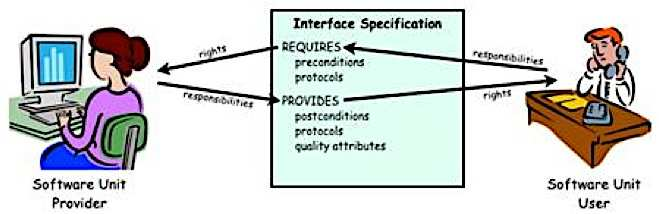
\includegraphics[width=0.8\linewidth]{design_by_contract.png}
\end{figure}

\subsection{Assertions}

\begin{description}
    \item[Function pre-conditions] required when the function is invoked
    \item[Function post-conditions] ensured when the function is terminated
    \item[Invariants] ensured at initialization and after every (public) function invocation
    \item[Protocols] Required and ensured constraints on invocations (eg open/close db connection)
    \item[Quality attribute] ensured by all functions
\end{description}

\subsection{Exceptions used to weaken pre-conditions}

Weaken preconditions allow to improve generality by making a software
unit more universally applicable. Precondition limit the applicability
of a method, by using exception, you can simplify the preconditions, by
catching exception rather than require some conditions at method
invocation. 

\begin{itemize}
\item Ex: function divide raise exception rather than check if divisor > 0.
    \end{itemize}

But not all preconditions can be handled in this way\ldots
